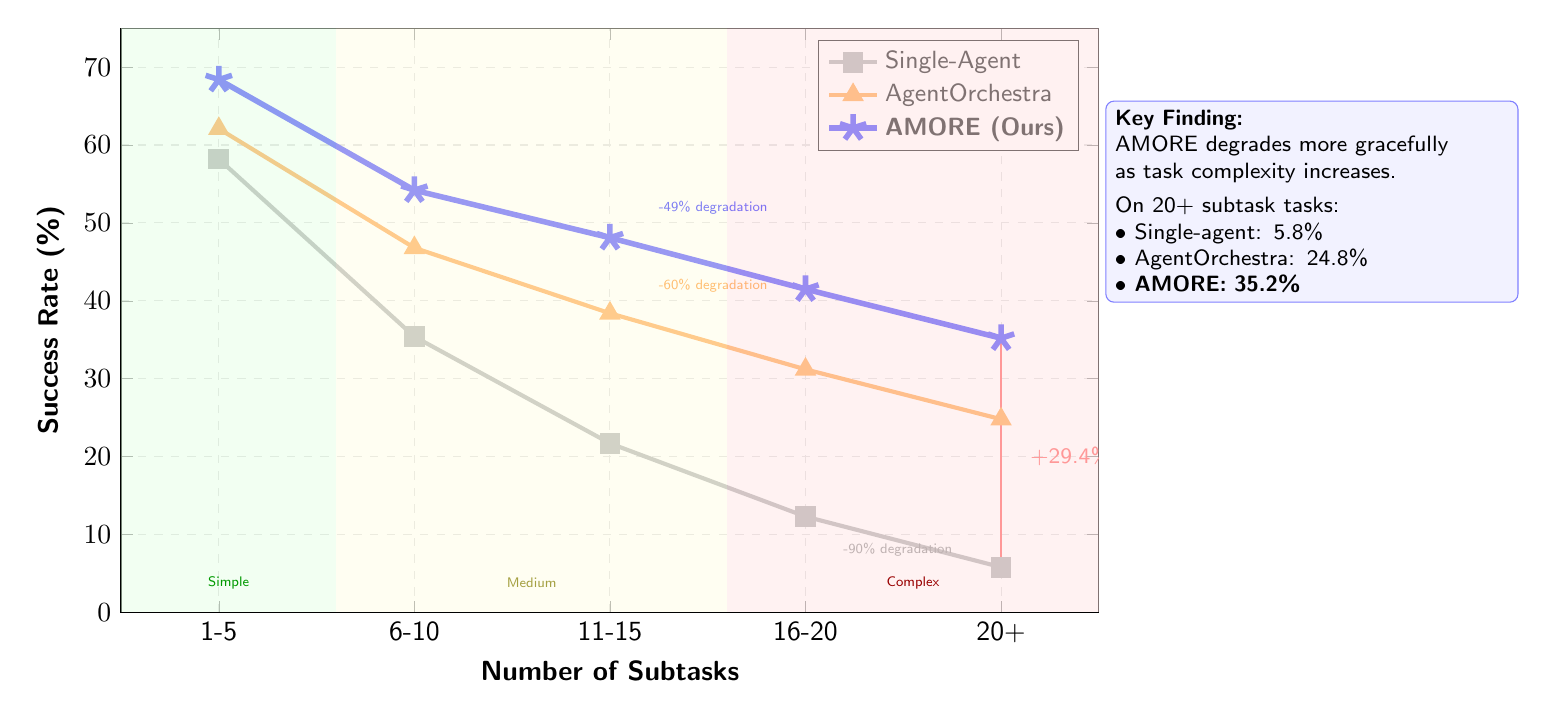
\begin{tikzpicture}
	\begin{axis}[
		width=14cm,
		height=9cm,
		xlabel={\textbf{Number of Subtasks}},
		ylabel={\textbf{Success Rate (\%)}},
		xmin=0.5,
		xmax=5.5,
		ymin=0,
		ymax=75,
		xtick={1,2,3,4,5},
		xticklabels={1-5, 6-10, 11-15, 16-20, 20+},
		ytick={0,10,20,30,40,50,60,70},
		grid=both,
		grid style={dashed, gray!30},
		ylabel style={font=\sffamily\bfseries},
		xlabel style={font=\sffamily\bfseries},
		tick label style={font=\sffamily},
%		title={\sffamily\bfseries\large Performance vs. Task Complexity (Number of Subtasks)},
		title style={yshift=8pt},
		legend style={
			at={(0.98,0.98)},
			anchor=north east,
			font=\sffamily\small,
			cells={anchor=west}
		}
		]
		% Single-Agent baseline
		\addplot[
		color=gray!70,
		mark=square*,
		mark size=3pt,
		line width=1.5pt
		] coordinates {
			(1, 58.2)
			(2, 35.4)
			(3, 21.7)
			(4, 12.3)
			(5, 5.8)
		};
		% AgentOrchestra
		\addplot[
		color=orange!80,
		mark=triangle*,
		mark size=3pt,
		line width=1.5pt
		] coordinates {
			(1, 62.1)
			(2, 46.8)
			(3, 38.4)
			(4, 31.2)
			(5, 24.8)
		};
		% AMORE
		\addplot[
		color=blue!80,
		mark=star,
		mark size=5pt,
		line width=2pt
		] coordinates {
			(1, 68.4)
			(2, 54.2)
			(3, 48.1)
			(4, 41.5)
			(5, 35.2)
		};
		\legend{Single-Agent, AgentOrchestra, \textbf{AMORE (Ours)}}
		% Annotations for key differences
		% Gap annotation at complex tasks
		\draw[<->, line width=1pt, color=red!70] (axis cs:5,5.8) -- (axis cs:5,35.2);
		\node[font=\sffamily\footnotesize, color=red!70, anchor=west] at (axis cs:5.1,20) {+29.4\%};
		% Degradation rates
		\node[font=\sffamily\tiny, color=gray, anchor=east, text width=2.5cm, align=right] at (axis cs:4.8,8) {-90\% degradation};
		\node[font=\sffamily\tiny, color=orange, anchor=west] at (axis cs:3.2,42) {-60\% degradation};
		\node[font=\sffamily\tiny, color=blue, anchor=west] at (axis cs:3.2,52) {-49\% degradation};
	\end{axis}
	% Insight box
	\node[draw=blue!50, fill=blue!5, rounded corners=3pt, font=\sffamily\footnotesize, text width=5cm, align=left, anchor=north west] at (12.5,6.5) {
		\textbf{Key Finding:}\\
		AMORE degrades more gracefully\\
		as task complexity increases.\\[3pt]
		On 20+ subtask tasks:\\
		\textbullet\ Single-agent: 5.8\%\\
		\textbullet\ AgentOrchestra: 24.8\%\\
		\textbullet\ \textbf{AMORE: 35.2\%}
	};
	% Complexity zone annotations
	\fill[green!10, opacity=0.5] (rel axis cs:0,0) rectangle (rel axis cs:0.22,1);
	\fill[yellow!10, opacity=0.5] (rel axis cs:0.22,0) rectangle (rel axis cs:0.62,1);
	\fill[red!10, opacity=0.5] (rel axis cs:0.62,0) rectangle (rel axis cs:1,1);
	\node[font=\sffamily\tiny, color=green!60!black] at (rel axis cs:0.11,0.05) {Simple};
	\node[font=\sffamily\tiny, color=yellow!60!black] at (rel axis cs:0.42,0.05) {Medium};
	\node[font=\sffamily\tiny, color=red!60!black] at (rel axis cs:0.81,0.05) {Complex};
\end{tikzpicture}